% Options for packages loaded elsewhere
\PassOptionsToPackage{unicode}{hyperref}
\PassOptionsToPackage{hyphens}{url}
\PassOptionsToPackage{dvipsnames,svgnames,x11names}{xcolor}
%
\documentclass[
  17pt,
  a4paper]{extarticle}
\usepackage{amsmath,amssymb}
\usepackage{lmodern}
\usepackage{iftex}
\ifPDFTeX
  \usepackage[T1]{fontenc}
  \usepackage[utf8]{inputenc}
  \usepackage{textcomp} % provide euro and other symbols
\else % if luatex or xetex
  \usepackage{unicode-math}
  \defaultfontfeatures{Scale=MatchLowercase}
  \defaultfontfeatures[\rmfamily]{Ligatures=TeX,Scale=1}
\fi
% Use upquote if available, for straight quotes in verbatim environments
\IfFileExists{upquote.sty}{\usepackage{upquote}}{}
\IfFileExists{microtype.sty}{% use microtype if available
  \usepackage[]{microtype}
  \UseMicrotypeSet[protrusion]{basicmath} % disable protrusion for tt fonts
}{}
\makeatletter
\@ifundefined{KOMAClassName}{% if non-KOMA class
  \IfFileExists{parskip.sty}{%
    \usepackage{parskip}
  }{% else
    \setlength{\parindent}{0pt}
    \setlength{\parskip}{6pt plus 2pt minus 1pt}}
}{% if KOMA class
  \KOMAoptions{parskip=half}}
\makeatother
\usepackage{xcolor}
\IfFileExists{xurl.sty}{\usepackage{xurl}}{} % add URL line breaks if available
\IfFileExists{bookmark.sty}{\usepackage{bookmark}}{\usepackage{hyperref}}
\hypersetup{
  pdftitle={RMarkdown, Bookdown or ClavertonDown?},
  pdfauthor={Emma Cliffe, Skills Centre: MASH},
  colorlinks=true,
  linkcolor={blue},
  filecolor={Maroon},
  citecolor={Blue},
  urlcolor={Blue},
  pdfcreator={LaTeX via pandoc}}
\urlstyle{same} % disable monospaced font for URLs
\usepackage[margin=2.5cm]{geometry}
\usepackage{longtable,booktabs,array}
\usepackage{calc} % for calculating minipage widths
% Correct order of tables after \paragraph or \subparagraph
\usepackage{etoolbox}
\makeatletter
\patchcmd\longtable{\par}{\if@noskipsec\mbox{}\fi\par}{}{}
\makeatother
% Allow footnotes in longtable head/foot
\IfFileExists{footnotehyper.sty}{\usepackage{footnotehyper}}{\usepackage{footnote}}
\makesavenoteenv{longtable}
\usepackage{graphicx}
\makeatletter
\def\maxwidth{\ifdim\Gin@nat@width>\linewidth\linewidth\else\Gin@nat@width\fi}
\def\maxheight{\ifdim\Gin@nat@height>\textheight\textheight\else\Gin@nat@height\fi}
\makeatother
% Scale images if necessary, so that they will not overflow the page
% margins by default, and it is still possible to overwrite the defaults
% using explicit options in \includegraphics[width, height, ...]{}
\setkeys{Gin}{width=\maxwidth,height=\maxheight,keepaspectratio}
% Set default figure placement to htbp
\makeatletter
\def\fps@figure{htbp}
\makeatother
\setlength{\emergencystretch}{3em} % prevent overfull lines
\providecommand{\tightlist}{%
  \setlength{\itemsep}{0pt}\setlength{\parskip}{0pt}}
\setcounter{secnumdepth}{5}
\newcommand{\BOO}{BOO}
\usepackage{float}
\ifLuaTeX
  \usepackage{selnolig}  % disable illegal ligatures
\fi

\title{RMarkdown, Bookdown or ClavertonDown?}
\author{Emma Cliffe, Skills Centre: MASH}
\date{}



%\usepackage[english,shorthands=off]{babel}
\usepackage{etoolbox}
\usepackage{spverbatim}
\makeatletter
\@ifpackageloaded{float}{}{\usepackage{float}}
\@ifpackageloaded{adjustbox}{}{\usepackage{adjustbox}}
\makeatother
\floatplacement{figure}{H}
\newcommand{\scalefactor}{1.7}
\adjustboxset*{min width=\scalefactor\width,max width=\linewidth}
\renewcommand{\familydefault}{phv}
\fontfamily{phv}\selectfont
\renewcommand{\em}{\bf}\renewcommand{\textit}{\textbf}\renewcommand{\emph}{\textbf}\renewcommand{\it}{\bf}\renewcommand{\itshape}{\bf}
\setlength{\parindent}{0.0pt}
\setlength{\parskip}{1.0\baselineskip}
\renewcommand{\baselinestretch}{1.5}\selectfont
\setlength{\mathsurround}{0.2em}
\setlength{\arraycolsep}{0.5cm}\renewcommand{\arraystretch}{1.5}
\addtolength{\jot}{\baselineskip}
\renewcommand{\;}{\,}
\sloppy
\allowdisplaybreaks
\usepackage{amsthm}
\newtheoremstyle{plain}{20pt}{3pt}{}{}{\bfseries}{.\newline\nobreak}{1.0em\nobreak}{}
\newtheoremstyle{definition}{20pt}{3pt}{}{}{\bfseries}{.\newline\nobreak}{1.0em\nobreak}{}
\newtheoremstyle{remark}{20pt}{3pt}{}{}{\bfseries}{.\newline\nobreak}{1.0em\nobreak}{}
\csundef{Proof}
\csundef{endProof}
\newenvironment{Proof}
  {\noindent{\bf Proof.}\hspace*{1em}}% Begin
  {\qed\par}% End
%% When redefining an environment it is vital that it has 
%% the same number of arguments as the original
\renewenvironment{proof}[1][\proofname]
  {\trivlist\item\relax\noindent{\bf {#1}.}\hspace*{1em}}% Begin
  {\qed\endtrivlist}% End

\begin{document}
\maketitle

{
\hypersetup{linkcolor=}
\setcounter{tocdepth}{2}
\tableofcontents
}
\newpage
\pagenumbering{arabic}

\hypertarget{an-introduction}{%
\section*{An introduction}\label{an-introduction}}
\addcontentsline{toc}{section}{An introduction}

\begin{itemize}
\tightlist
\item
  Requirements
\item
  Formats and transforms
\item
  Markdown
\item
  RMarkdown
\item
  Bookdown
\item
  Clavertondown
\end{itemize}

\hypertarget{requirements}{%
\section{Requirements}\label{requirements}}

\begin{itemize}
\tightlist
\item
  Public Sector Bodies (Websites and Mobile Applications) (No.~2) Accessibility Regulations requires at least one of:

  \begin{itemize}
  \tightlist
  \item
    \href{https://accessibilityinsights.io/docs/en/web/overview}{Web: WCAG 2.1 AA} + \href{https://docs.mathjax.org/en/v2.7-latest/misc/accessibility-features.html}{MathJax!}
  \item
    \href{https://support.office.com/en-gb/article/make-your-word-documents-accessible-to-people-with-disabilities-d9bf3683-87ac-47ea-b91a-78dcacb3c66d}{Word 365: Accessibility checker + Equation editor}
  \item
    \href{https://support.microsoft.com/en-us/office/make-your-powerpoint-presentations-accessible-to-people-with-disabilities-6f7772b2-2f33-4bd2-8ca7-dae3b2b3ef25}{PowerPoint 365: Accessibility checker + Equation editor}
  \item
    \href{https://docs.mathjax.org/en/v2.7-latest/misc/epub.html}{EPub3 with MathML}
  \end{itemize}
\item
  Equality Act 2010

  \begin{itemize}
  \tightlist
  \item
    Authors may need to provide additional formats to meet the needs of a specific student
  \item
    Not all screenreaders or other assistive technology can read all accessible formats e.g.~you may need to produce Word on request even if you decide not to provide this to meet the Public Sector Boddies act.
  \end{itemize}
\end{itemize}

\hypertarget{formats-and-transforms}{%
\section{Formats and transforms}\label{formats-and-transforms}}

\begin{figure}
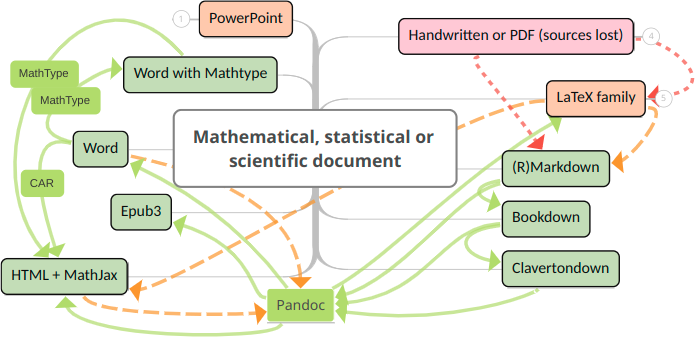
\includegraphics[width=1\linewidth]{map} \caption{Accessible and interactive map at https://www.mindomo.com/mindmap/document-transforms-2d8186b662758e26ccf50ef82a3828b2}\label{fig:unnamed-chunk-1}
\end{figure}

\hypertarget{markdown}{%
\section{Markdown}\label{markdown}}

``Markdown is a text-to-HTML conversion tool for web writers. Markdown allows you to write using an easy-to-read, easy-to-write plain text format, then convert it to structurally valid XHTML (or HTML).''

John Grubber, Markdown creator
\url{https://daringfireball.net/projects/markdown/}

\hypertarget{rmarkdown}{%
\section{RMarkdown}\label{rmarkdown}}

\begin{itemize}
\tightlist
\item
  Simple one page documents containing maths and/or statistics
\item
  RStudio provides a GUI interface
\item
  Multiple output formats with consistent structure

  \begin{itemize}
  \tightlist
  \item
    Accessible: HTML, Word
  \item
    Accessible if no mathematical content: ODT, RTF
  \item
    Inaccessible: LaTeX/PDF
  \item
    Slides

    \begin{itemize}
    \tightlist
    \item
      Possibly accessible: PowerPoint, HTML using ioslides, reveal.js, Slidy
    \item
      Inaccessible: LaTeX/Beamer
    \end{itemize}
  \end{itemize}
\end{itemize}

For further information on getting started, an example and how to test for accessibility at \href{https://stem-enable.github.io/RMarkdownWorkshop/}{RMarkdown Workshop}

\hypertarget{bookdown}{%
\section{Bookdown}\label{bookdown}}

\begin{itemize}
\tightlist
\item
  Designed to enable authors of \textbf{books} or longer structured documents
\item
  Needed for:

  \begin{itemize}
  \tightlist
  \item
    Parts and appendices
  \item
    Finer control of figures
  \item
    Automatic numbering and cross-referencing of figures and tables with captions
  \item
    Cross referencing of pieces of text
  \item
    Equation numbering and referencing
  \item
    Theorem and proof environments with numbering and referencing
  \item
    Definition of custom environments
  \item
    Citation management via Pandoc, biblatex or natbib
  \item
    Embedding of web pages and HTML widgets
  \end{itemize}
\item
  Output to HTML book, LaTeX/PDF and EPub3 only

  \begin{itemize}
  \tightlist
  \item
    Multiple output formats but structure may be inconsistent e.g.~numbering is internally consistent but may differ between formats
  \end{itemize}
\end{itemize}

\hypertarget{clavertondown}{%
\section{ClavertonDown}\label{clavertondown}}

\begin{itemize}
\tightlist
\item
  Designed to enable authors of \textbf{lecture notes} to meet the diverse needs of students by production of a consistent \textbf{set} of formats
\item
  Needed for:

  \begin{itemize}
  \tightlist
  \item
    Bookdown features but with transformation to Word
  \item
    Flexible theorem-like environments akin to amsthm package in LaTeX including consistent styling, numbering and classification of type across multiple output formats

    \begin{itemize}
    \tightlist
    \item
      Numbering system of inbuilt Bookdown theorems can be changed
    \item
      Internal references within theorem names and captions
    \item
      Unnumbered theorem environments with original numbering
    \item
      Shared numbering e.g.~between theorem and proposition
    \item
      Newtheorem-type definition of theorem-like environments
    \item
      Repeating theorem-like environments
    \end{itemize}
  \item
    Inclusion of figures in knitr engine based custom blocks, including all theorem-like, while still allowing transform to Word
  \item
    Supplied limited controls over visual presentation to enable a coherent set of notes with

    \begin{itemize}
    \tightlist
    \item
      Known accessibility features
    \item
      Clear visual markers of structure including structured colour for theorem-like environments in non-PDF formats
    \end{itemize}
  \end{itemize}
\item
  Output as a mini-linked site of a set of formats which can include HTML book, HTML page, Word, EPub3, standard PDF, clear print PDF and large print PDF
\end{itemize}

\hypertarget{made-at-claverton-down}{%
\section{Made at Claverton Down}\label{made-at-claverton-down}}

ClavertonDown is built by MASH, if you need something to work differently we may be able to adapt it for you. However, you should only use ClavertonDown if you cannot achieve what you need using Bookdown as going back requires you to undo all use of extra features!

\begin{itemize}
\tightlist
\item
  \href{https://bathmash.github.io/clavertondown/}{ClavertonDown}
\item
  \href{https://www.bath.ac.uk/projects/mathematics-accessibility/}{MASH Accessible Maths project}
\end{itemize}

\end{document}
